\begin{figure}[ht]
    \begin{subfigure}[t]{.15\textwidth}
        \caption{}
        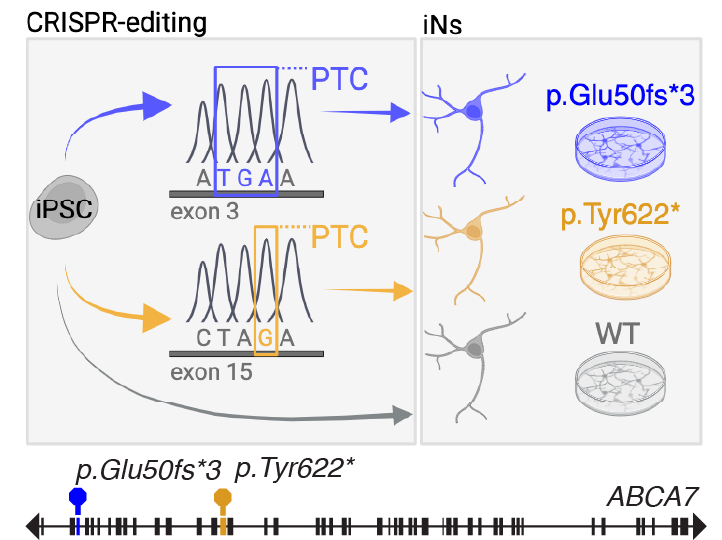
\includegraphics[width=\textwidth]{./main_plots/iN_cartoon.png}        
    \end{subfigure}    %\includegraphics[width=\textwidth]{figS1.png}
    \begin{subfigure}[t]{.15\textwidth}
        \caption{}
        \includegraphics[width=\textwidth]{./main_plots/iN_image.png}        
    \end{subfigure}  
    \begin{subfigure}[t]{.15\textwidth}
        \caption{}
        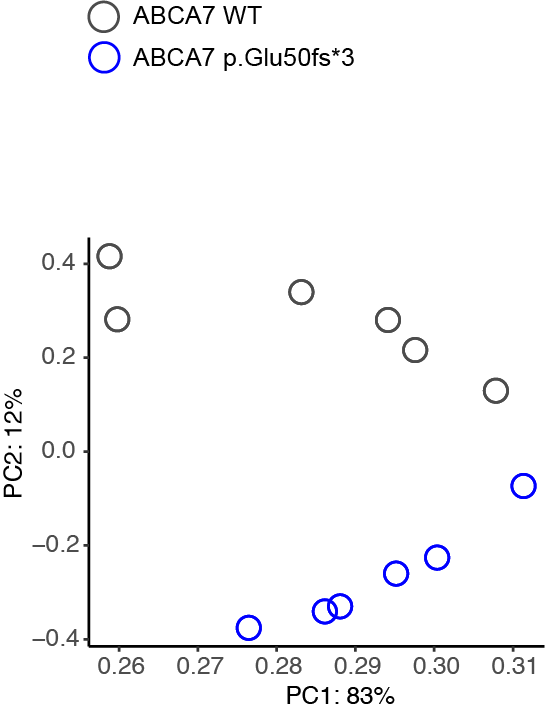
\includegraphics[width=\textwidth]{./main_plots/g2_pca_lipids.png}        
    \end{subfigure}  
    \begin{subfigure}[t]{.5\textwidth}
        \caption{}
        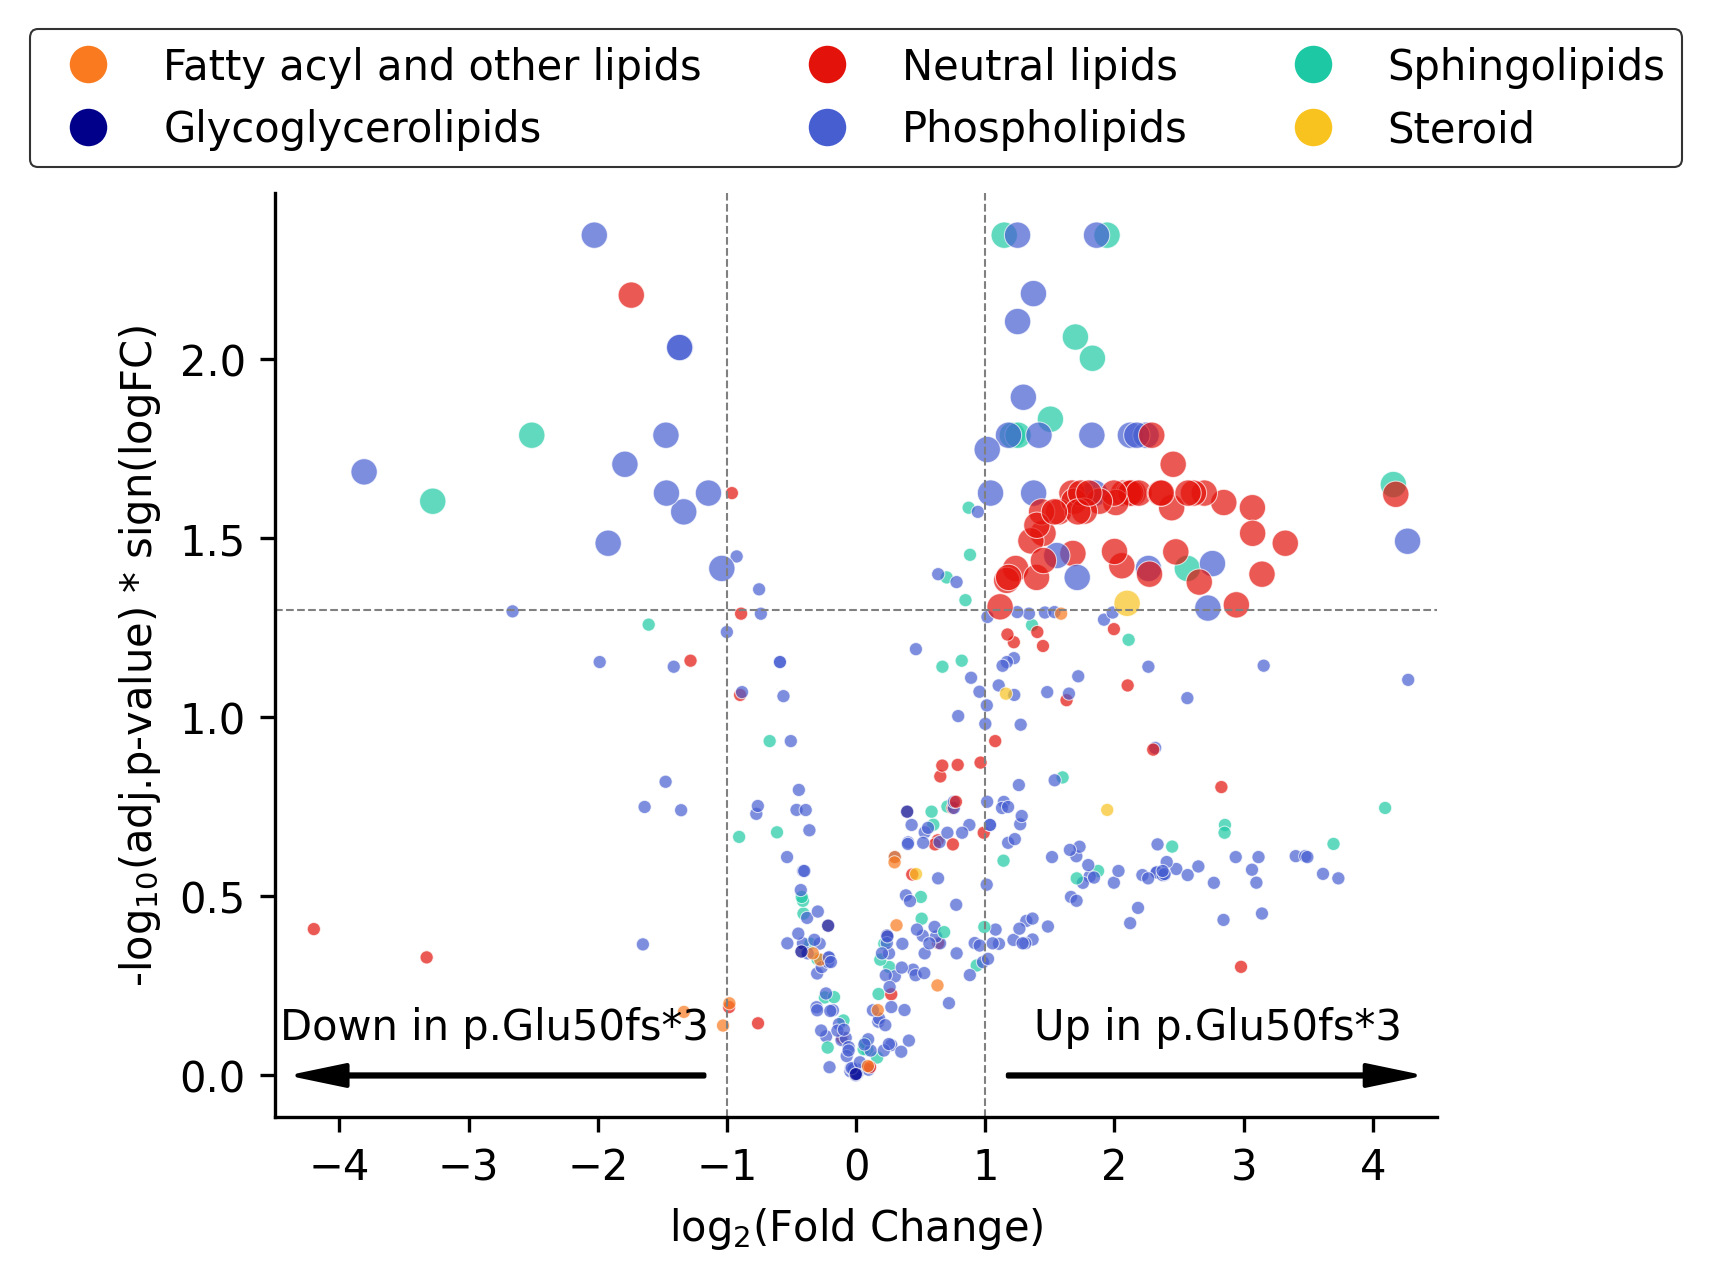
\includegraphics[width=\textwidth]{./main_plots/iN_lipids_overview.png}        
    \end{subfigure}   
    \begin{subfigure}[t]{.24\textwidth}
        \caption{}
        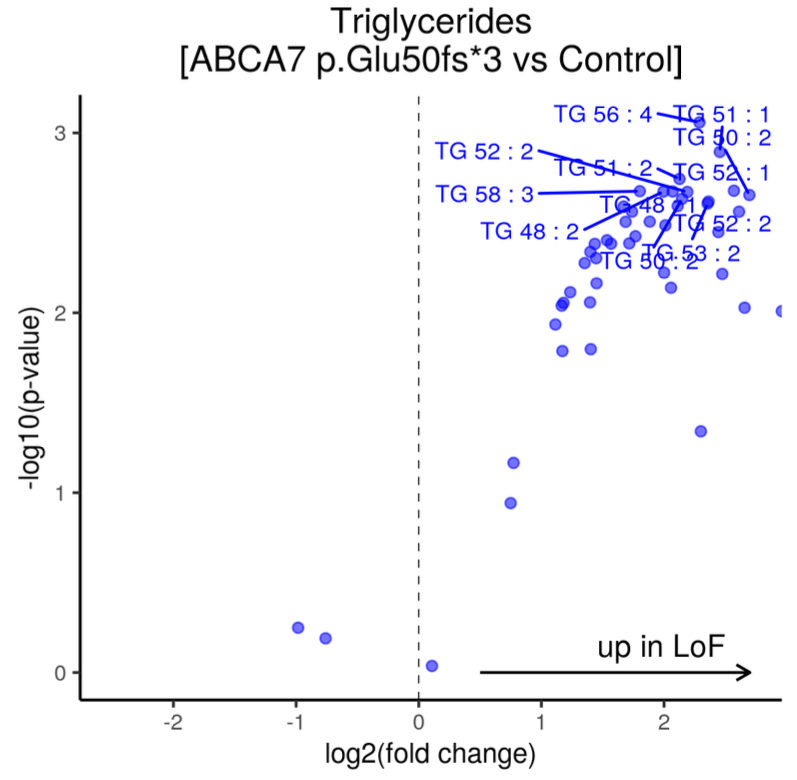
\includegraphics[width=\textwidth]{./main_plots/tg_volcano.png}        
    \end{subfigure} 
    \begin{subfigure}[t]{.24\textwidth}
        \caption{}
        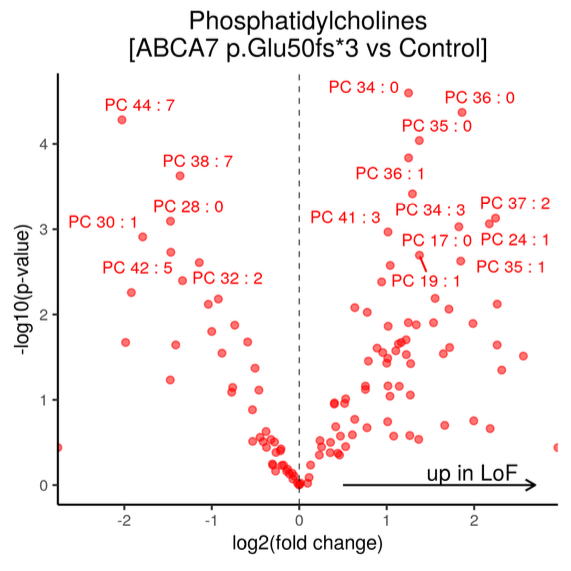
\includegraphics[width=\textwidth]{./main_plots/pc_volcano.png}        
    \end{subfigure} 
    \begin{subfigure}[t]{.24\textwidth}
        \caption{}
        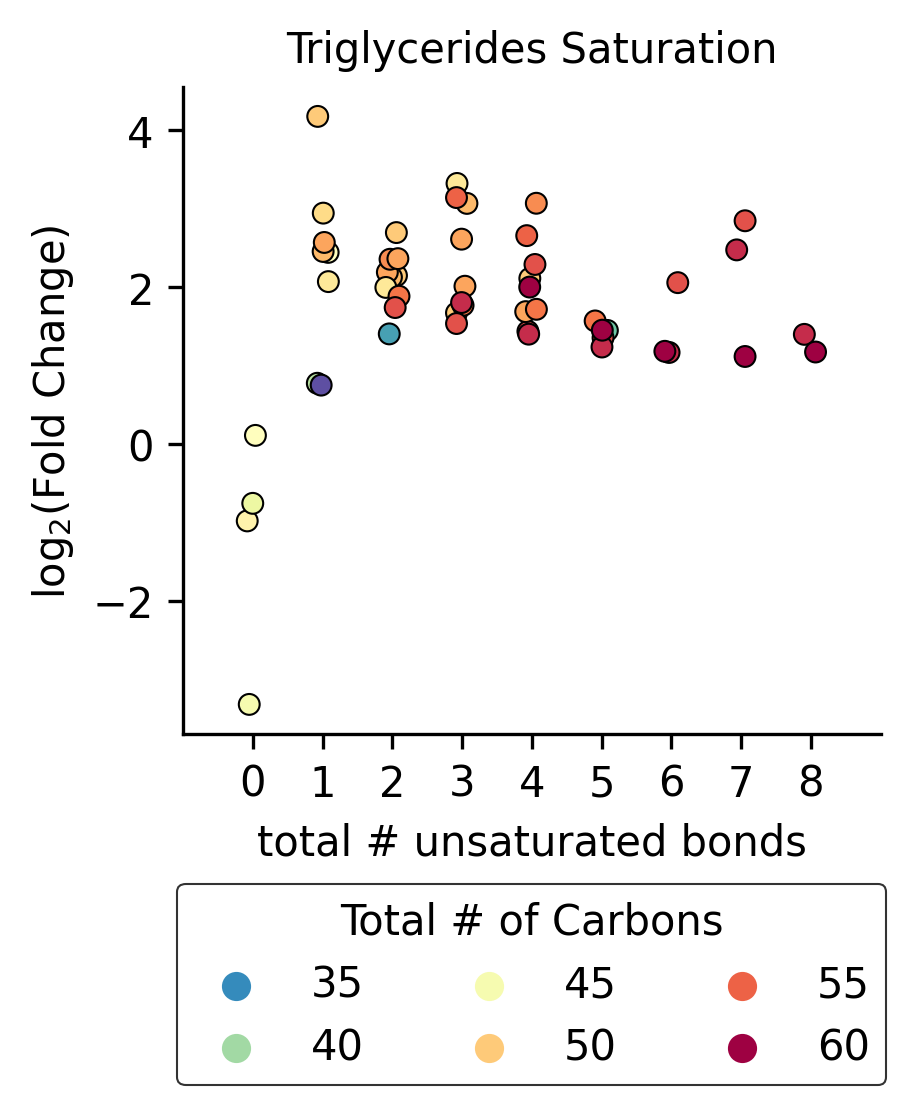
\includegraphics[width=\textwidth]{./main_plots/TG_saturation.png}        
    \end{subfigure} 
    \begin{subfigure}[t]{.24\textwidth}
        \caption{}
        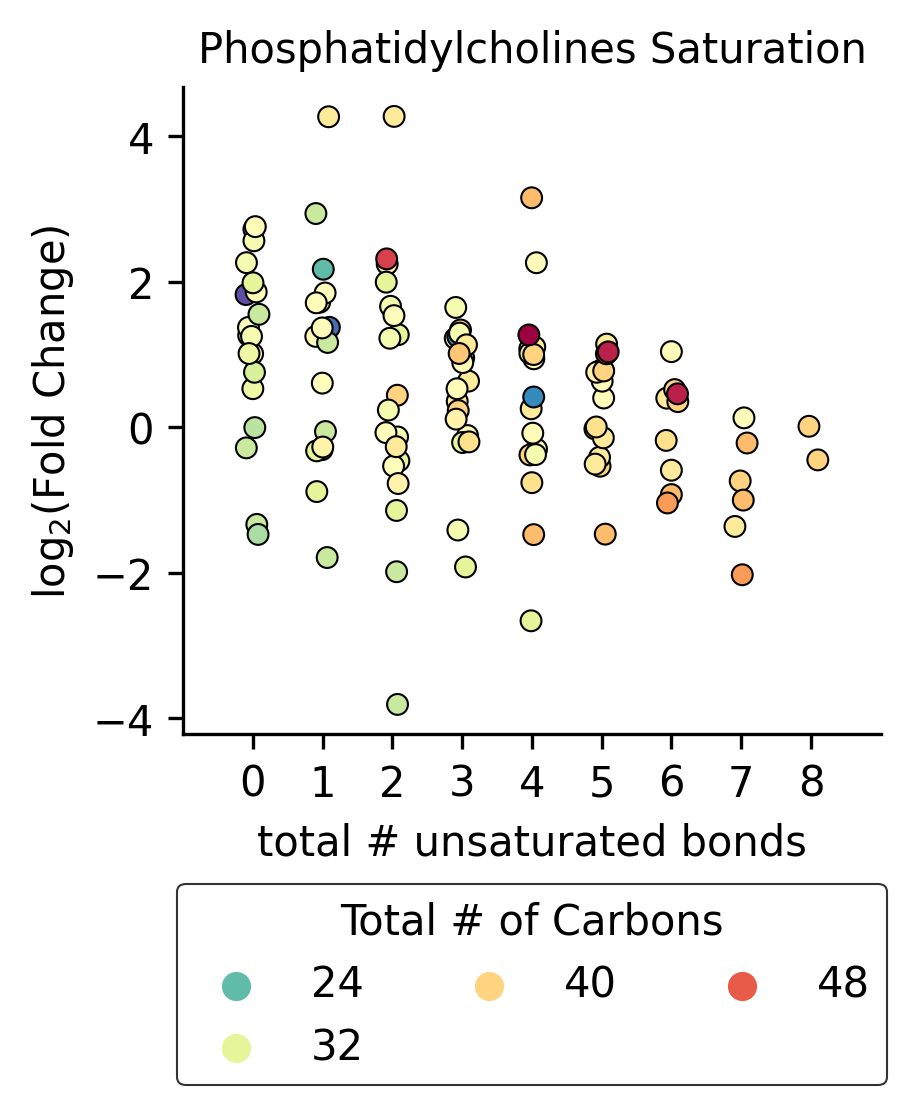
\includegraphics[width=\textwidth]{./main_plots/PC_saturation.png}        
    \end{subfigure} 
    \caption{
        \textbf{ABCA7 LoF Neurons Have Neutral Lipid Accumulation and Phospholipid Imbalances.}\\[1ex]
        (A) Volcano plot showing the distribution of lipid species by log-fold-change and log-p-value, where log-fold-change > 0 indicates up-regulation in ABCA7 LoF post-mortem PFC (N=8) vs. Control (N=8). A subset of lipid species is labeled ($p<0.1$ \& logFC>0.5 (red) or logFC<-0.5 (blue)) (p-values by independent sample t-test). 
        (B) Overview of two iPSC-derived isogenic neuronal lines carrying ABCA7 LoF variants. ABCA7 gene map depicts exons (black rectangles) and introns (black lines). 
        (C) CRISPR-Cas9 was used to generate an ABCA7 LoF isogenic iPSC line by introducing a premature termination codon into exon 3 or exon 15 (ABCA7 p.Glu50fs*3, blue or p.Tyr622*, orange, respectively). 
        (D) Example MAP2 staining of 2-week-old p.Tyr622* iNs. 
        (E) Representative sweeps show action potentials elicited by 800 ms of current injections in patched 4-week-old iNs. 
        (F) Summary of action potential frequency (means ± SEM) elicited with different amounts of injected current in 4-week-old iNs. 
        (G) Projection of control and ABCA7 p.Glu50fs*3 lipidomes (per-sample z-scaled peak areas; $N=6$ per genotype) onto the first two principal components from lipid space. Fraction of explained variance shown along each axis. 
        (H) Volcano plot showing perturbed lipid species by class (p-values by independent sample t-test). 
        (I) Overview of perturbed lipid species by lipid subclass. $U =$ number of lipids in that subclass where $p<5 \times 10^{-3}$ \& fold-change > 0. $D =$ number of lipids in that subclass where $p<5 \times 10^{-3}$ \& fold-change < 0. $T = U + D$. \% = ($T/N$)$\times 100$, where $N =$ total number of lipids in a given subclass (p-values by independent sample t-test; $N=6$ per genotype). (J,K) Volcano plot showing the distribution of triglyceride (TG) species 
        (J) and phosphatidylcholine (PC) species (K) by log-fold-change and log-p-value, where log-fold-change > 0 indicates up-regulation in p.Glu50fs*3 ($N=6$) vs. WT ($N=6$) iPSC-derived neurons. A subset of lipid species is labeled ($p<0.05$ \& logFC>2 (red) or logFC<-2 (blue)) (p-values by independent sample t-test). 
        (L) Schematic of metabolic link between TG, monoglyceride (MG), and diglyceride (DG). 
        (M-Q) Relative abundance of select lipid species in p.Glu50fs*3 iN ($N=6$) and WT iN ($N=6$) (p-values by independent sample t-test). Boxes indicate per-condition dataset quartiles, and whiskers extend to the most extreme data points not considered outliers (i.e., within 1.5 times the interquartile range from the first or third quartile). (R) Schematic from (L) overlaid with abundance changes in p.Glu50fs*3 iNs vs. WT iNs. Schematics in (C, L, R) created with BioRender.com.
    }
    \label{fig:main_lipids}
\end{figure}